\documentclass{article}
\usepackage[utf8]{inputenc}
\usepackage{amsmath}
\usepackage{listings}
\usepackage{xcolor}
\usepackage{geometry}
\usepackage{graphicx}
\usepackage{tikz}
\usepackage{url}
\geometry{margin=1in}
\title{Spreadsheet Engine with Vim Integration}
\author{Ayushmaan Pandey 2021EE30709 \\
Aryanshu Lawania 2023CS10279 \\
Shubh Chhabra 2021EE10645}

\date{\today}

\begin{document}

\maketitle

\section{Overview}
This project is a spreadsheet engine implemented in Rust, designed with extensibility, encapsulation, and interactive control in mind. It supports formula computation, undo/redo, cell formatting, and integrates a Vim-style interface for text navigation and editing.

An extension of the system includes a Vim-inspired spreadsheet interface that allows cursor movement, insert mode, formatting commands, and command-mode navigation, mimicking the experience of a terminal-based text editor while manipulating structured spreadsheet data.
\footnote{Source code available at: \url{https://github.com/Asterisk07/Rust-Lab-Spreadsheet-program}}

\section{Design Choices and Justification}

\subsection{Modular Architecture}
The system is broken down into multiple Rust modules: formulas, graph, parser, vim, etc. Each has a clearly defined responsibility, promoting encapsulation and separation of concerns.

\textbf{Justification}: This design enables parallel development and unit testing, and keeps the codebase scalable and maintainable.

\subsection{Dependency Graph for Formulas}
Dependencies between cells are managed using a directed graph. When a formula is updated, the graph is modified and a topological sort determines the order of recomputation.

\textbf{Justification}: This ensures efficient and accurate recomputation, avoids redundant calculations, and handles cyclic dependencies gracefully.

\subsection{Transaction-based Undo/Redo}
The Vim module maintains a transaction history using stacks of cell state changes.

\textbf{Justification}: This is an effective way to implement undo/redo while preserving cell history in a minimal and efficient form.

\subsection{Vim Editor Integration}
A VimEditor struct encapsulates cursor movement, input buffering, and mode switching. Terminal events are handled using the crossterm crate for cross-platform support.

\textbf{Justification}: Mimicking Vim enhances user experience for terminal users, and it keeps the interface consistent with the modal editing paradigm.

\section{Module Graph Overview}
Below is a visual representation of how different modules in the system are structured and depend on each other:

\begin{center}
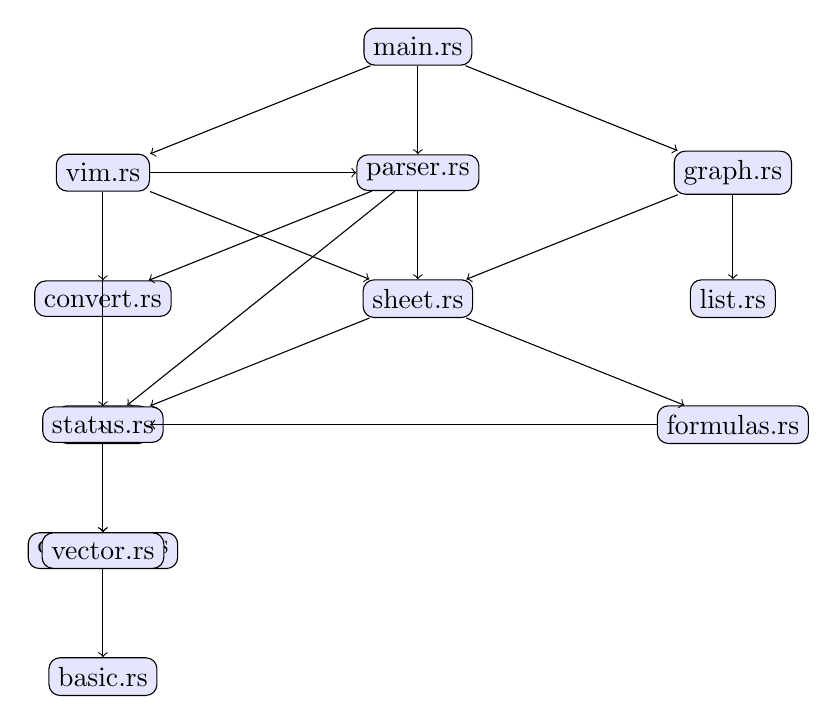
\begin{tikzpicture}[node distance=1.6cm, every node/.style={draw, rounded corners, fill=blue!10}]
  \node (main) {main.rs};
  \node (vim) [below of=main, xshift=-4cm] {vim.rs};
  \node (parser) [below of=main, xshift=0cm] {parser.rs};
  \node (graph) [below of=main, xshift=4cm] {graph.rs};
  
  \node (sheet) [below of=parser, xshift=0cm] {sheet.rs};
  \node (info) [below of=sheet, xshift=-4cm] {info.rs};
  \node (formulas) [below of=sheet, xshift=4cm] {formulas.rs};
  
  \node (list) [below of=graph] {list.rs};
  \node (convert) [below of=vim] {convert.rs};
  \node (status) [below of=convert] {status.rs};
  \node (compare) [below of=status] {compare.rs};
  \node (vector) [below of=info] {vector.rs};
  \node (basic) [below of=compare] {basic.rs};

  % Arrows for dependencies
  \draw[->] (main) -- (vim);
  \draw[->] (main) -- (parser);
  \draw[->] (main) -- (graph);
  \draw[->] (parser) -- (sheet);
  \draw[->] (graph) -- (sheet);
  \draw[->] (vim) -- (sheet);
  \draw[->] (vim) -- (convert);
  \draw[->] (vim) -- (status);
  \draw[->] (vim) -- (parser);
  \draw[->] (sheet) -- (info);
  \draw[->] (sheet) -- (formulas);
  \draw[->] (formulas) -- (info);
  \draw[->] (graph) -- (list);
  \draw[->] (parser) -- (convert);
  \draw[->] (parser) -- (info);
  \draw[->] (info) -- (status);
  \draw[->] (info) -- (vector);
  \draw[->] (status) -- (compare);
  \draw[->] (compare) -- (basic);
\end{tikzpicture}
\end{center}

Each node in the diagram represents a module:
\begin{itemize}
  \item \textbf{basic.rs} - low-level utilities
  \item \textbf{compare.rs} - custom comparison logic
  \item \textbf{formulas.rs} - spreadsheet functions like SUM, AVG
  \item \textbf{info.rs} - cell metadata and formula configuration
  \item \textbf{main.rs} - entry point for launching the application
  \item \textbf{sheet.rs} - manages the 2D cell grid
  \item \textbf{vector.rs} - low-level math functions
  \item \textbf{convert.rs} - A1-style label and index conversion
  \item \textbf{graph.rs} - dependency tracking and topological sort
  \item \textbf{list.rs} - memory-managed linked list for graph edges
  \item \textbf{parser.rs} - parses input and expressions
  \item \textbf{status.rs} - tracks global and cell statuses
  \item \textbf{vim.rs} - interactive terminal UI with Vim controls
\end{itemize}

\section{Data Structures Used}
\begin{itemize}
  \item \textbf{Adjacency List} (in graph.rs) to model cell dependencies.
  \item \textbf{Stacks} for undo/redo history (in vim.rs).
  \item \textbf{HashMap} to map cell indices to expressions.
  \item \textbf{2D Vector} of CellFormat to store cell styles.
  \item \textbf{Function Pointer Table} to dispatch formula operations.
\end{itemize}

\section{Encapsulation Techniques}
Encapsulation is achieved through:
\begin{itemize}
  \item \textbf{Private fields and helper methods} for internal state management.
  \item \textbf{Modular separation} of parsing (parser.rs), formula execution (formulas.rs), dependency management (graph.rs), and UI (vim.rs).
  \item \textbf{CommandInfo and Info structs} to isolate the data exchanged between modules.
\end{itemize}

\section{Vim-Based Spreadsheet Extension}
The Vim extension provides:
\begin{itemize}
  \item Movement using h, j, k, l OR arrow keys
  \item Editing mode with i, ESC
  \item Command mode with commands like  :h, :b, :i, :u, :color red, :reset
  
\end{itemize}

\textbf{Help Menu Example:}
\begin{lstlisting}
MOVEMENT:
  h, j, k, l -> Move cursor
EDITING:
  i -> Insert mode
COMMANDS:
  :b -> Bold
  :i -> Italic
  :u -> Underline
  :color red -> Set color
  :reset -> Clear formatting
\end{lstlisting}

Note : 
\begin{itemize}
  \item Using formatting command twice (:b, :i, :u) removes it.
  \item Formatting commands can be cascaded (i.e. :b and :u and color can be applied at once).
  
\end{itemize}
\section{Undo-Redo Extension}
\begin{itemize}
  \item We added undo and redo features into the autograder extension activated by "undo" and "redo" commands.
  \item Also availaible in vim mode by ":undo" or ":redo"
  
\end{itemize}

\section{Challenges Faced}
\begin{itemize}
  \item \textbf{Rust's Ownership Model}: Handling shared mutable access, particularly with RefCell and Rc, was a recurring complexity.
  \item \textbf{Integrating Vim UI with Spreadsheet Logic}: Bridging modal input handling with spreadsheet computations required careful design.
  \item \textbf{Recursive Updates}: Ensuring that dependent cell updates are consistent and cyclic dependencies are detected.
\end{itemize}

\section{Limitations and Future Improvements}
\begin{itemize}
  \item \textbf{Cell Grid Rendering}: Improve UI by drawing grid lines to better visualize individual cells.
  % \item \textbf{String Support}: Currently, cells only support integer values. Extending to support strings is a future goal.
  % \item \textbf{Complex Formulas}: Extend formula language to support functions like \texttt{MIN(A1:A3)+B1}.
  \item \textbf{Command Suggestions}: Auto-suggest commands or support fuzzy matching in command mode.
\end{itemize}

% \section{Unimplemented Extensions}
% % (Leave this for user to fill in later)

% \begin{itemize}
%  \item \texttt{:select <value>} → Highlight all matches of that value : We realised too late that in the current structure (the info struct with the value that can be both explicit (numerical) or a expression) would be too difficult to implement a reverse-hashing based search.
%   \item \textt{yxr/ yxc} →  Cut row/column :  We did expect issues in deleting a row or column as that would require shifting rows and columns entirely and we thought we could iterate over the sheet with somethinig like sheet[x][y] = sheet[x+1][y], however actually fixing the issues turned out to be more complicated than this and we ran out of time trying to fix it.
%   \item \texttt{x} → Delete cell : Similar as cut row/column       
%         \item \texttt{yyr/yyc} → Copy row/column : Copying wasnt the main issue, but pasting was, so we decided to leave out copying as well.
%         \item \texttt{p} → Paste row or column : Pasting posed similar issue as cutting since here too we had initally thought to do like sheet[x+1][y] = sheet[x][y] but it turned out too complex.
%   \item \texttt{Writing to csv} → Writing to csv using :w command. : We were able to imeplement writing to csv for numerical spreadsheet, but couldnt solve the problem of properly writing into csv the spreadsheet while properly storing the expressions in encoded form, and so instead of implementing this feature and then hoping the user doesnt use expressions in the sheet, we decided to scrap this entirely.
%   % \item \textbf{String Support}: 
%   \item \texttt{Complex Formulas}→ Extend formula language to support functions like \texttt{MIN(A1:A3)+B1} : Would require re-implementing the entire graph struct and all formulas code since we couldnt reuse the autograder formulas.rs , so we skipped this due to lack of time and low ROI.
%   \item \texttt{Chart Generation} : We felt this to be too trivial so prioritized this less.

%   Great raw draft — let’s clean this up into something polished but still natural and candid, like the rest of a project report. I’ll preserve your reasoning and structure but tweak phrasing, grammar, and flow for clarity:

% ---

\section{Unimplemented Extensions}

\begin{itemize}
 \item \texttt{:select <value>} → Highlight all matches of that value:  
 We realized too late that in our current design — where each cell’s value in the \texttt{info} struct could either be an explicit numerical value or an expression — implementing an efficient reverse-lookup would be difficult. It would have required a reverse-hashing or indexing mechanism which wasn’t feasible within our current structure.

 \item \texttt{yxr / yxc} → Cut row/column:  
 We anticipated that deleting a row or column would require shifting the remaining cells accordingly, and initially planned to handle this by iterating over the sheet with something like \texttt{sheet[x][y] = sheet[x+1][y]}. However, during implementation we ran into unexpected edge cases and complications in maintaining formula dependencies and references, and ultimately ran out of time attempting to resolve these.

 \item \texttt{x} → Delete cell:  
 This faced similar issues as cutting rows or columns. Shifting cells and maintaining formula consistency turned out to be more involved than initially expected.

 \item \texttt{yyr / yyc} → Copy row/column:  
 Copying in itself wasn’t difficult — the challenge was pasting the copied data correctly while preserving relative references and dependencies. Since pasting was left incomplete, we decided to leave out copying as well for consistency.

 \item \texttt{p} → Paste row or column:  
 Pasting ran into the same structural challenges as cutting, since our naive idea of shifting cells with \texttt{sheet[x+1][y] = sheet[x][y]} turned out to be insufficient for handling formulas and reference updates. This too was dropped due to time constraints.

 \item \texttt{Writing to csv} → Writing to CSV using the \texttt{:w} command:  
 While we managed to implement CSV export for purely numerical spreadsheets, handling expressions in a clean, encoded form for the CSV turned out to be non-trivial. Rather than implementing a partial, unreliable solution (which would silently fail if the user happened to use expressions), we chose to omit this feature entirely.

 \item \texttt{Complex Formulas} → Extend formula language to support functions like \texttt{MIN(A1:A3)+B1}:  
 Implementing this would have required reworking the formula parser and dependency graph from scratch, as we couldn’t reuse the \texttt{formulas.rs} module provided by the autograder. Given the high effort and relatively low impact on overall functionality, we skipped this due to time constraints.

 \item \texttt{Chart Generation}:  
 We considered this a low-priority, somewhat trivial feature compared to core spreadsheet operations, and hence deprioritized it in favor of more fundamental functionalities.
\end{itemize}

  % \item \textbf{Command Suggestions}: Auto-suggest commands or support fuzzy matching in command mode.
% \end{itemize}

\end{document}